\subsection{Angular Velocity Observer Comparative \\
                Numerical Simulation Study}
\label{chSMS_ID.sec.AVO_sim}

\begin{center}
\begin{figure}[htbp]
  \begin{center}
%    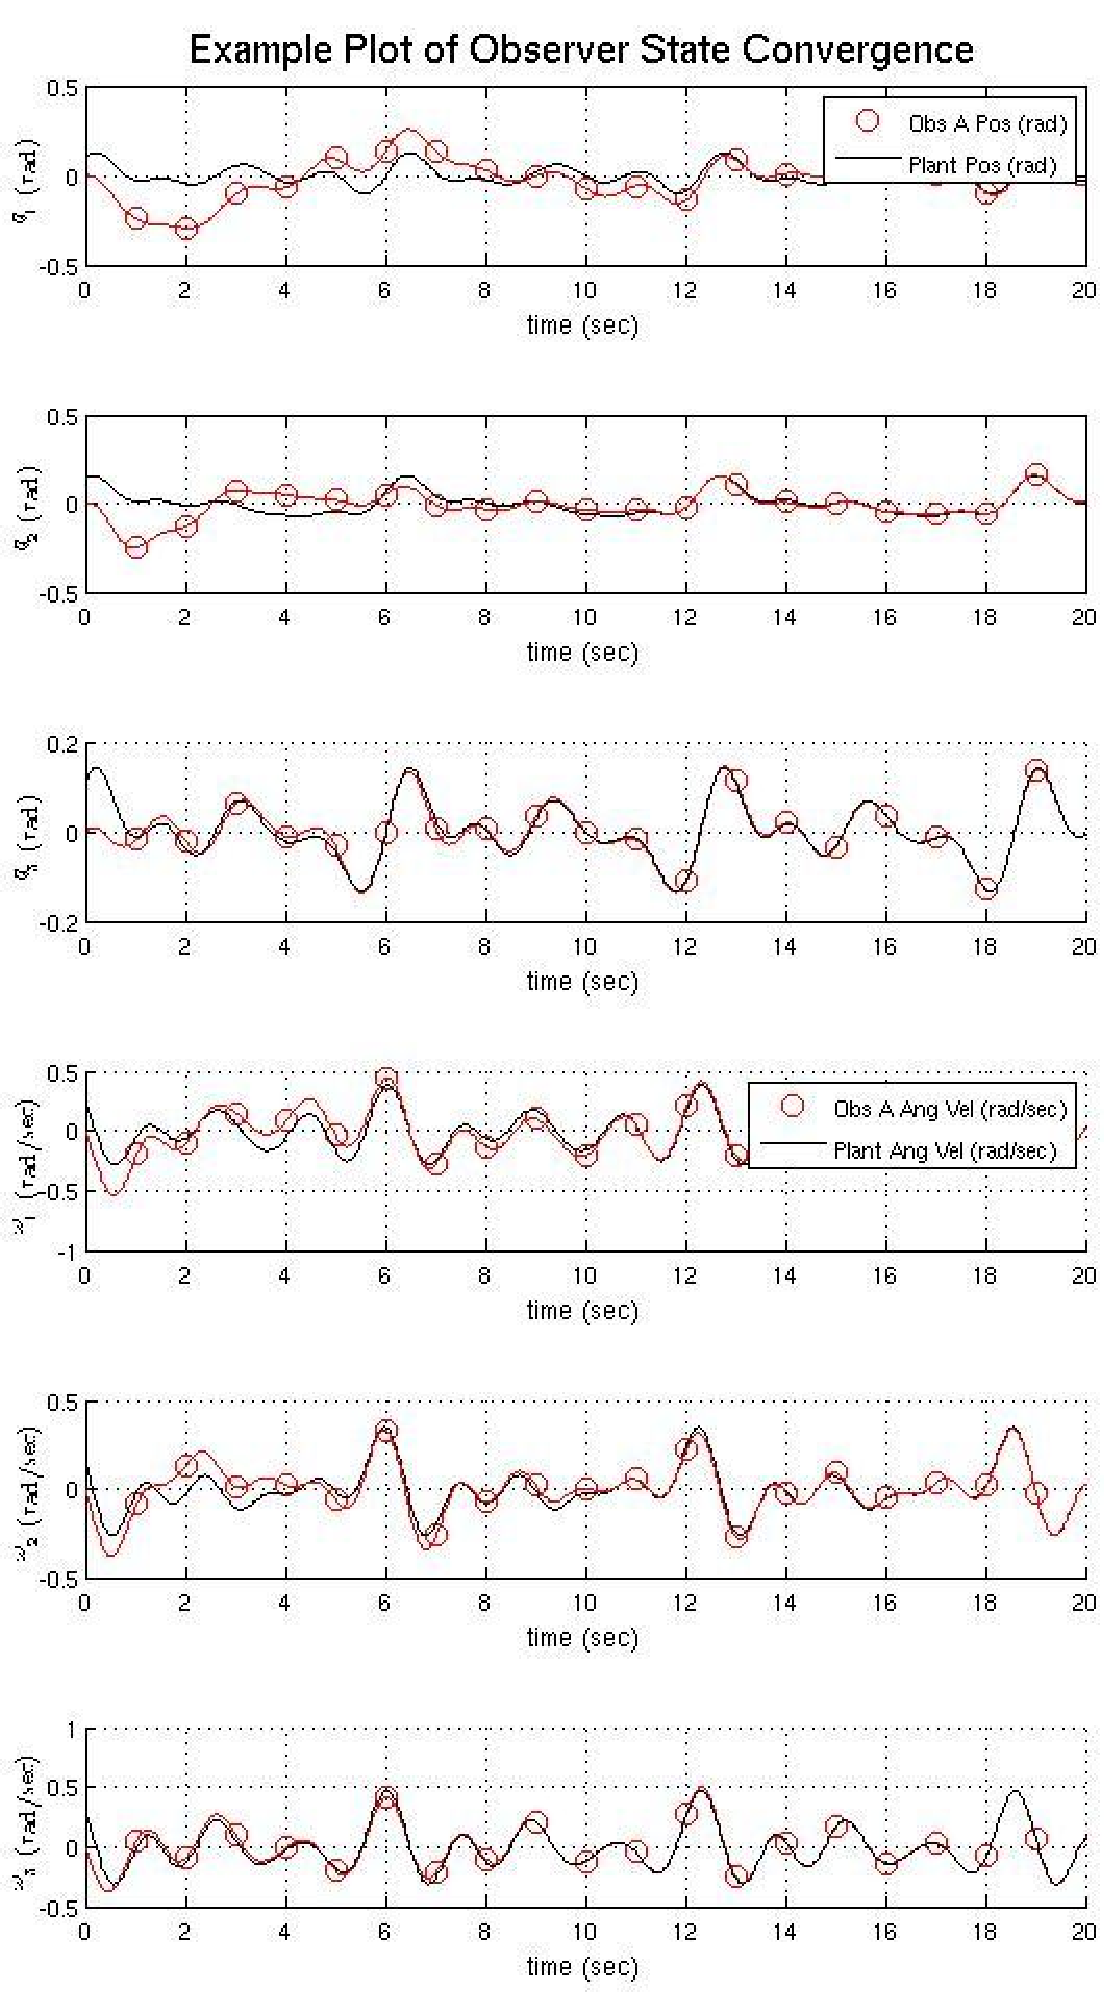
\includegraphics[width=110mm]{./chSMS_ID/images/nextFull3}
    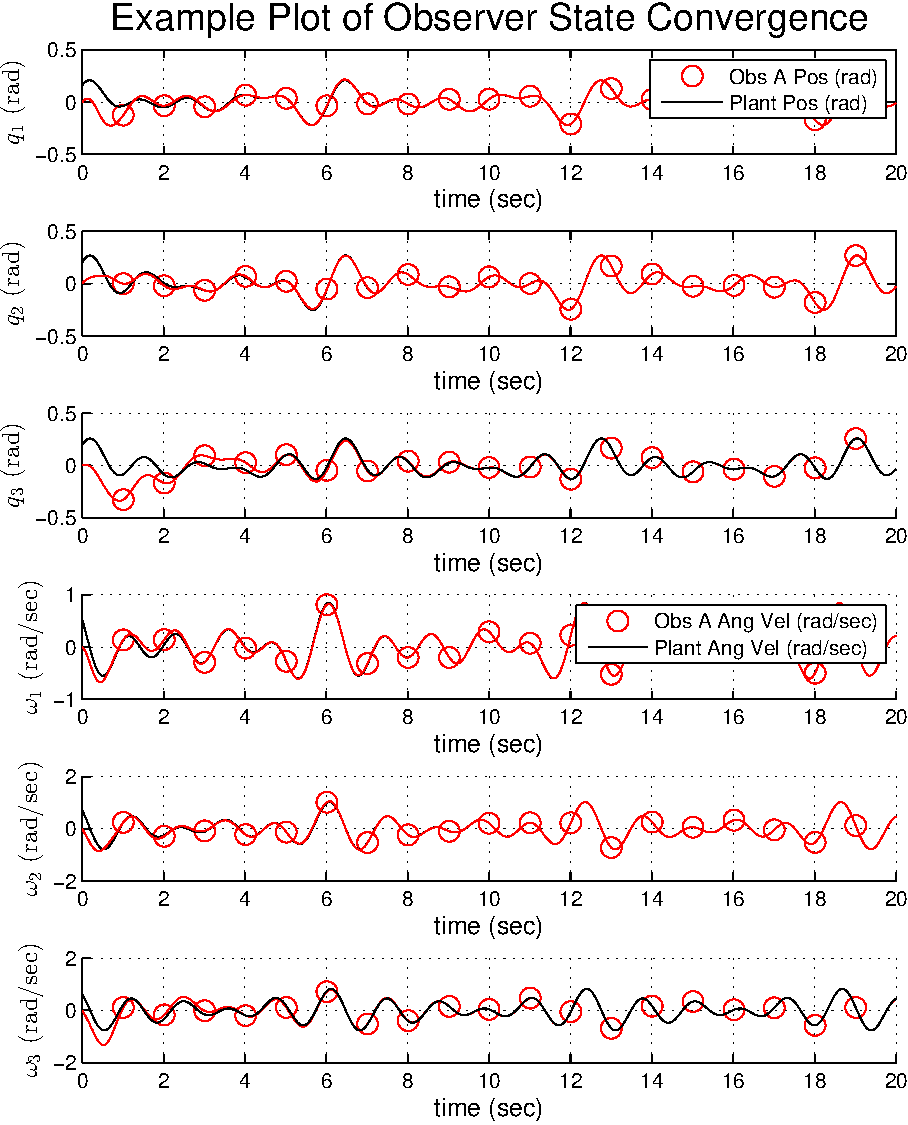
\includegraphics[width=150mm]{./chSMS_ID/images/jhuObsStateConv}
    %{./images/jhuObsFig}
  \end{center}
  \caption{ Angular position and angular velocity simulation the
    plant, (\ref{chModels.eq.SO3plant}), and Observer A,
    (\ref{chSMS_ID.eq.AVO}).  Note convergence of Observer A state to
    plant state in each of the 6 \ac{DOF}.}
  \label{chSMS_ID.fig.AVO}
\end{figure}
\end{center}

This Section reports a comparative analysis of numerical simulations
for the three angular velocity observers described in Sections
\ref{chSMS_ID.sec.AVO}, \ref{chSMS_ID.sec.AVO_Sal}, and
\ref{chSMS_ID.sec.AVO_TT}. We assume the plant's inertia tensor, $I$,
is known and the signals of the plant rotational position, $q(t)$, and
the plant torque input, $\tau(t)$, are available.

Each observer's performance was evaluated numerically using
a fourth order Runge-Kutta numerical solution
with fifth order error control. In every case during simulation
the initial state of the observer was $\hat{q}(0)=\vec{0}$ and
$\hat{\omega}(0)=\vec{0}$. 

Plant position trajectories and control inputs satisfying
(\ref{chModels.eq.SO3plant}) were generated numerically.  Plant position
trajectories, $q(t)$, were generated analytically as a sum of sines
and cosines, each with different frequencies and amplitudes, such that
$\|q(t)\|<\frac{\pi}{2}$.  Corresponding plant velocity signals
$\dot{q}(t)$ and $\omega(t)$ were similarly generated analytically.
Plant signals $\dot{\omega}(t)$ and $\tau(t)$ were computed
numerically. In this simulation study we report
\begin{itemize}
\item the body-frame observer (\ref{chSMS_ID.eq.AVO}) as Observer A, 
\item the world-frame observer (\ref{chSMS_ID.eq.AVO_Sal}) as  Observer B, and
\item the coordinate free observer (\ref{chSMS_ID.eq.AVO_TT}) as Observer C.
\end{itemize}

Feedback gains appearing in the three observers differ in form and
dimension.  In an effort to achieve a fair comparison, we chose
observer gains such that, when the observer error systems were
linearized about the equilibrium point $\Delta q=\Delta \bar{q}=\Delta
\tilde{q}=\vec{0}$ and $\Delta \omega=\vec{0}$, the resulting
linearized gain terms were approximately equal.  Equality was be
achieved for the linearized error dynamics of Observers A and B.  The
gains of Observer C, which differ in structure from A and B, were set
such that the average of the eigenvalues of the gain matrices of its
linearized error dynamics were equal to the average eigenvalue of the
gain matrices of the linearized error dynamics of both Observers A and
B. Given $k\in\mathcal{R}$ such that $k>0$ then each observer was
proven to be locally convergent to the plant's state and the gain
equivalence described was achieved by using the following formulas
%
\vspace{5mm}
\begin{itemize}
\item $E=(\frac{k}{2})I^{-1}$ Observer A
\item $k_p=1$ and $k_v=k$ Observer B
\item $\alpha=\frac{k}{4}g_{avg}$ and $\beta=\frac{1}{2}g_{avg}$ for
   Observer C
\end{itemize}
%
where $g_{avg}$ is the average of the eigenvalues of $I^{-1}$.

To evaluate and compare differences in observer convergence we
simulated a number of scenarios.  For observer gains such that $k>0$,
all three observers were seen to be asymptotically stable (i.e. state
estimates converged to the state of the plant).  For example Figure
\ref{chSMS_ID.fig.AVO} shows a typical case of Observer A converging
to the plant's state in all six \ac{DOF}. Figure
\ref{chSMS_ID.fig.AVO_allNorm} is a sample plot showing the magnitude
of angular position error and angular velocity error with respect to
time for all three observers.  For simulations of plants with
inertia tensor eigenvalues near or less than 1.0, the three
observers seemed to converge in a similar fashion. However, Figure
\ref{chSMS_ID.fig.AVO_allNorm} shows Observer B displaying
under-damped behavior which slows its convergence.  This behavior
diminished as either the gain is increased or the inertia is lowered.
Figure \ref{chSMS_ID.fig.AVO_avgNorm2} shows the average of 50 trials
with inertia tensor eigenvalues less than unity and, on average, you
can see the similar behavior of the different velocity
observers.

\begin{center}
\begin{figure*}[htbp]  
  \begin{center}
    %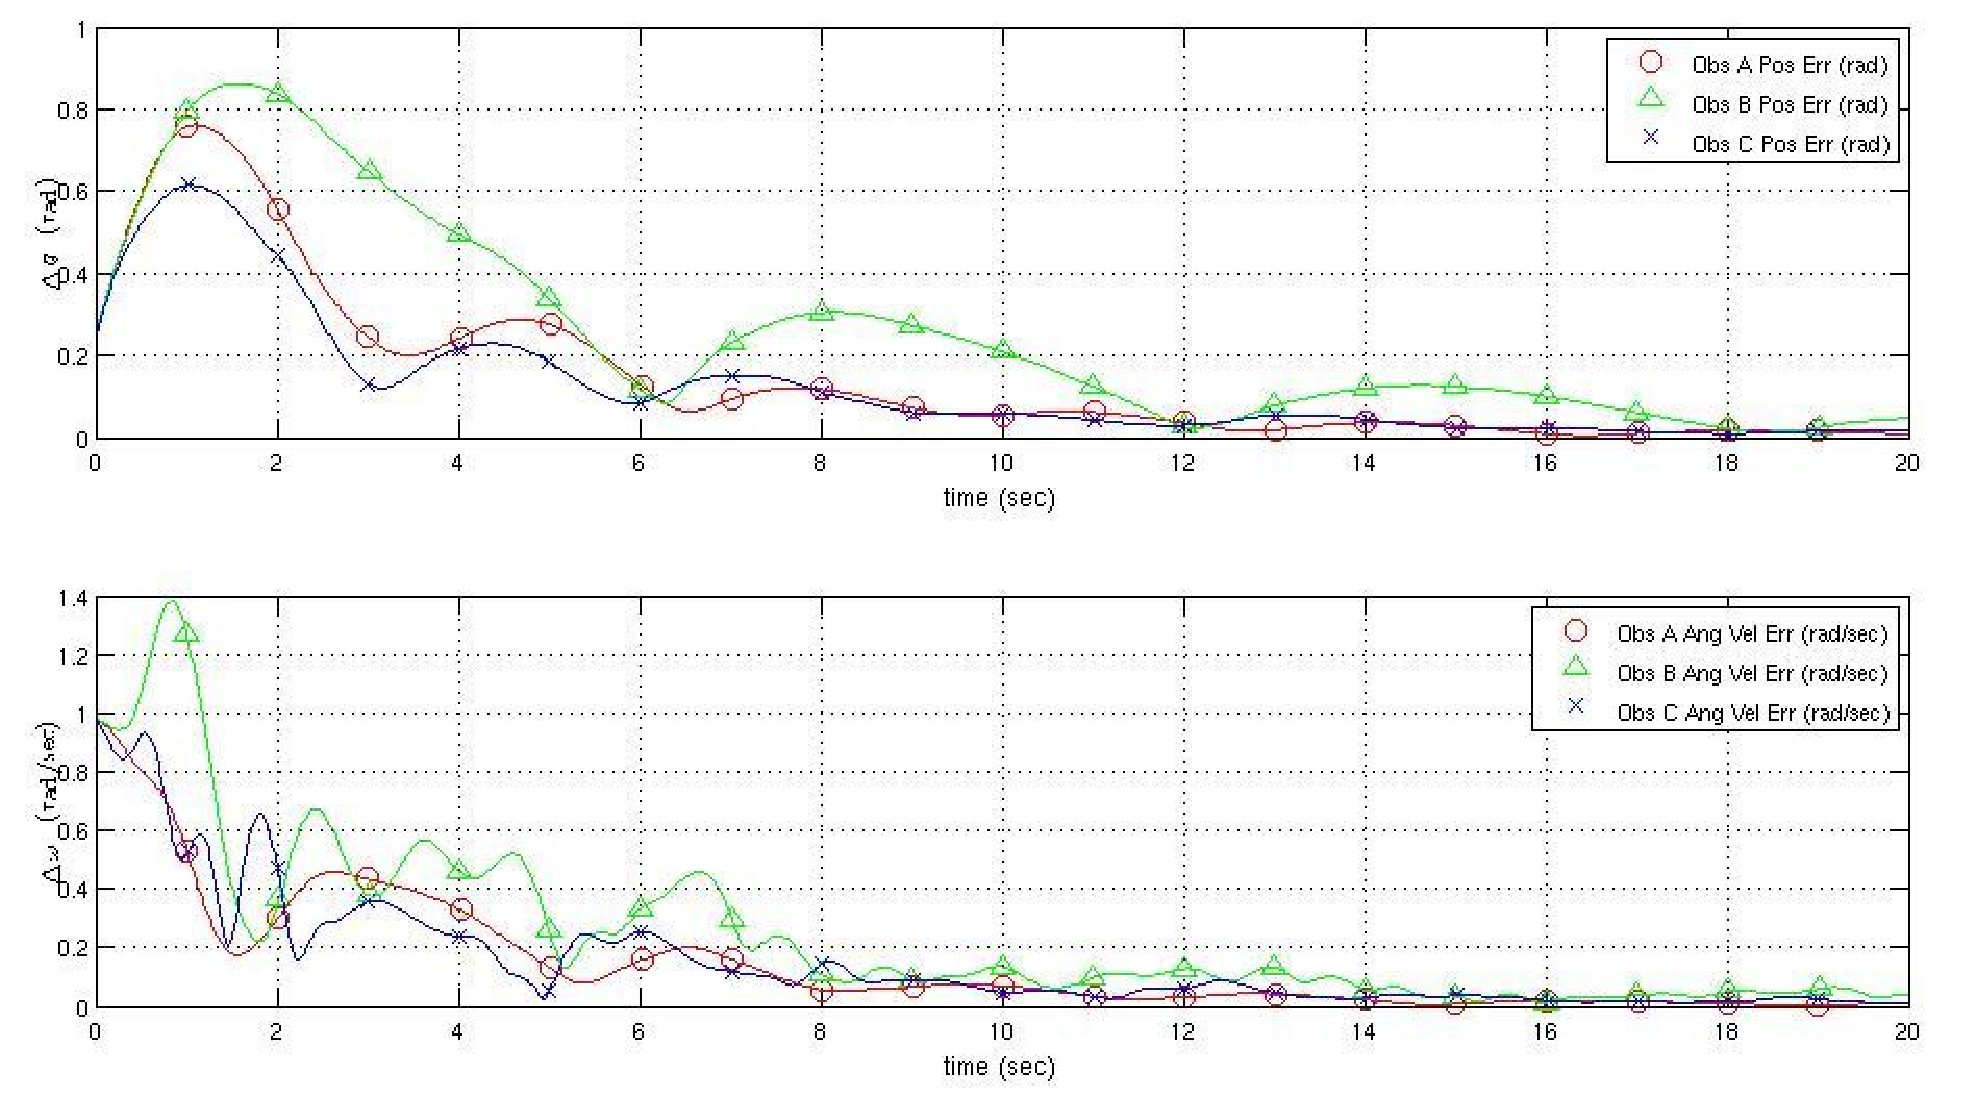
\includegraphics[width=150mm]{./chSMS_ID/images/nextExErr2}%{./images/allNormFig}
    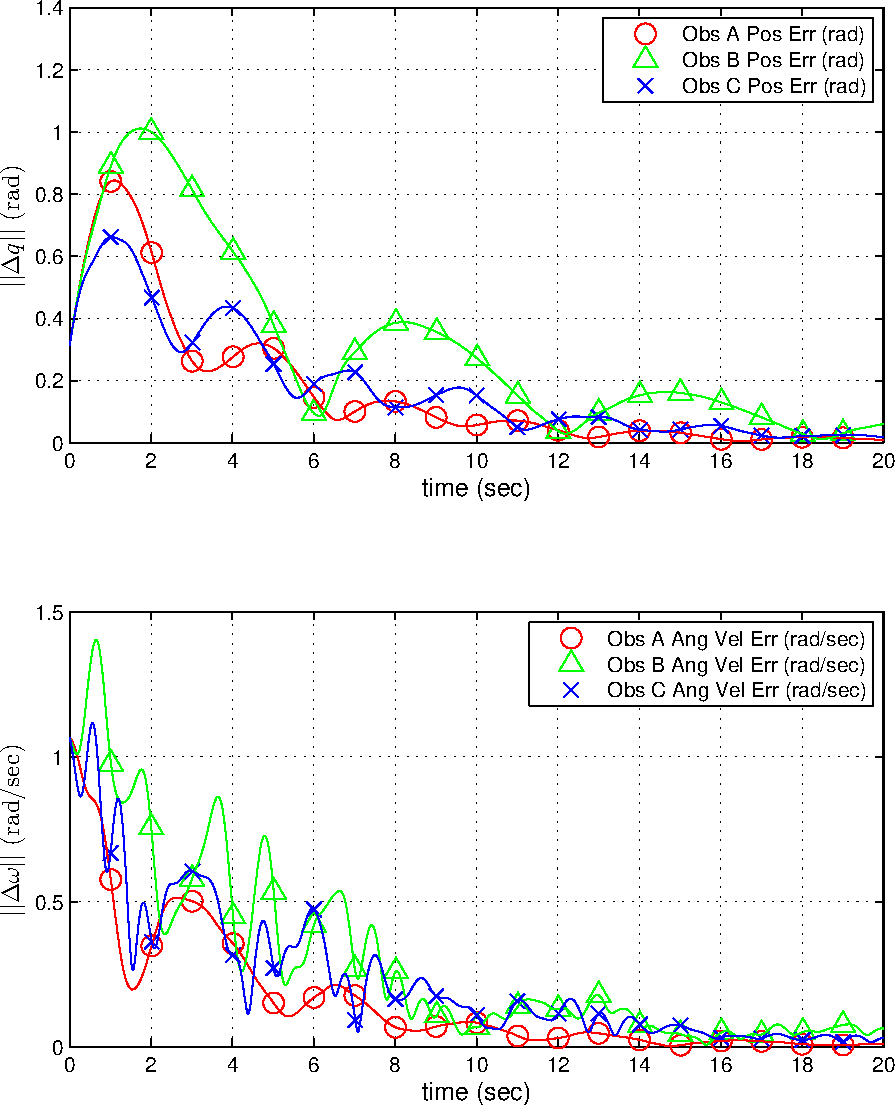
\includegraphics[width=150mm]{./chSMS_ID/images/obsNormErrPlot}%{./images/allNormFig}
  \end{center}
  \caption{Rotational error magnitude and angular velocity error
    magnitude between observer state and plant state.}
  \label{chSMS_ID.fig.AVO_allNorm}
\end{figure*}
\end{center}

\begin{center}
\begin{figure*}[htbp]
  \begin{center}
%    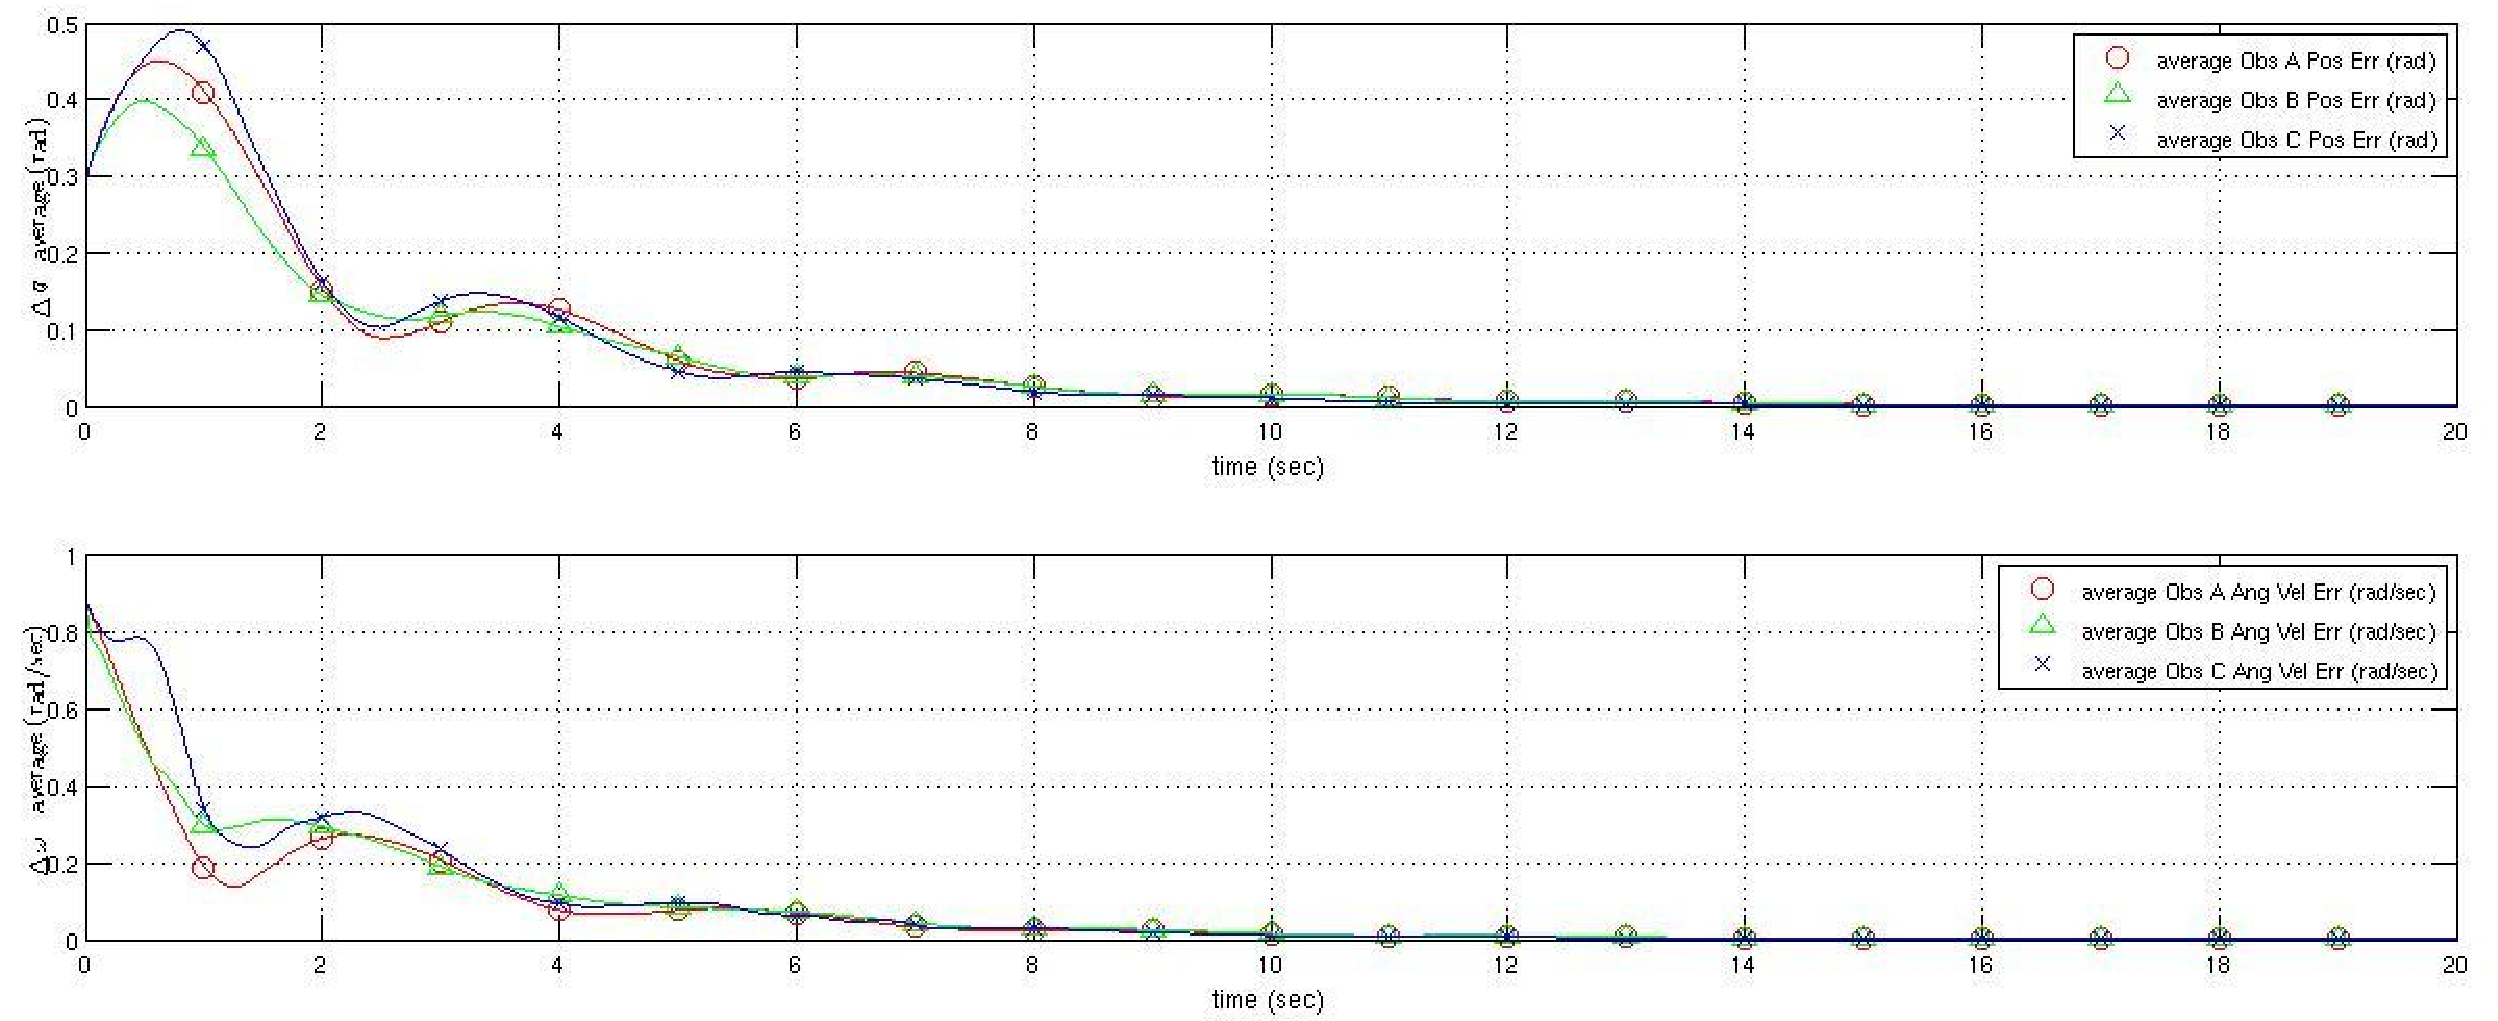
\includegraphics[width=150mm]{./chSMS_ID/images/nextAvgErr2}
    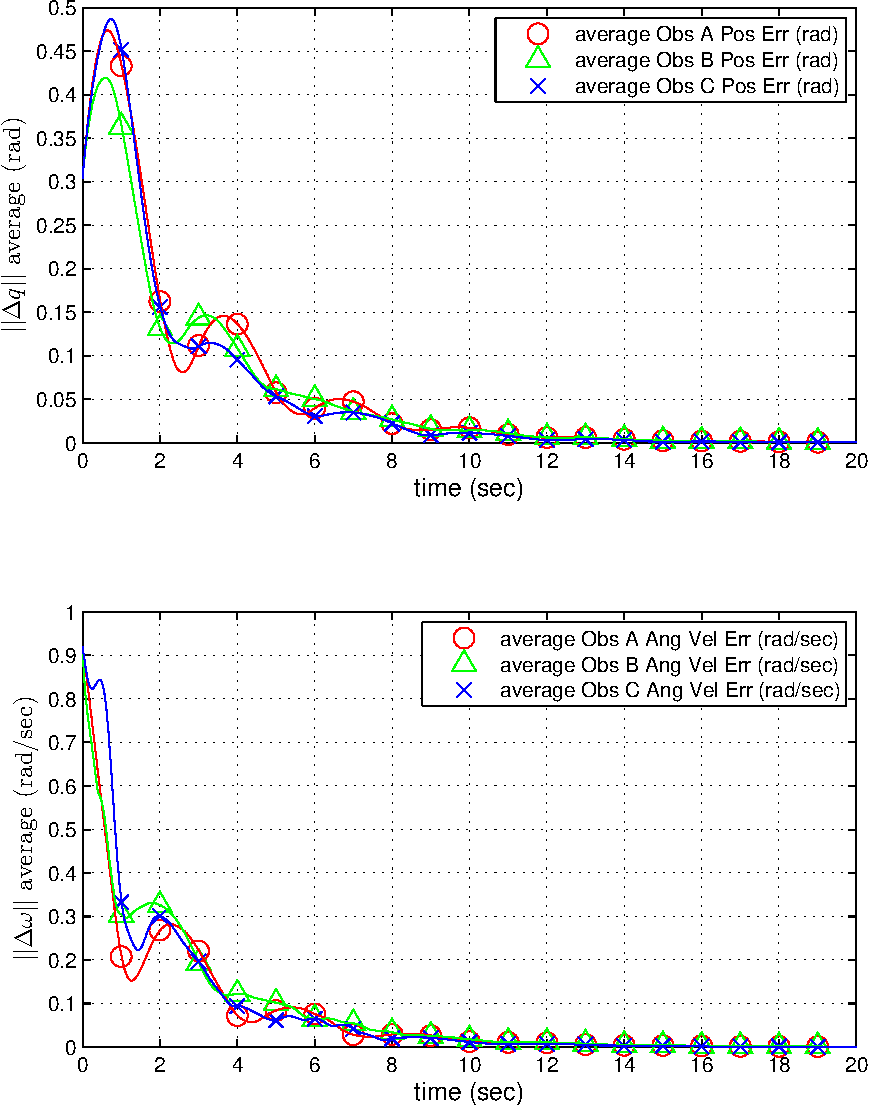
\includegraphics[width=150mm]{./chSMS_ID/images/allObsAvgErr}
  \end{center}
  \caption{Average rotational error magnitude and average angular
    velocity error magnitude between observer state and plant state of
    an ensemble of 50 randomized angular position profile trials and
    inertia tensor eigenvalues less than one.}
  \label{chSMS_ID.fig.AVO_avgNorm2}
\end{figure*}
\end{center}



